\chapter{Difusión del Proyecto}

Dada la practicidad del proyecto y que existe realmente una demanda del mismo (limitada pero existente) se han llevado a cabo diversas actividades para conseguir la máxima difusión del mismo:

\begin{itemize}
  \item Página Web del proyecto.
  
  \item Publicación en la Google Play.
  
  \item Mantenimiento del repositorio en GitHub.
  
  \item Difusión en la página oficial de la biblioteca INDI.
  
  \item Difusión en el foro oficial de la biblioteca INDI.
\end{itemize}

En las siguientes secciones se comentan más en detalle cada una de dichas actividades.

\section{Página Web del Proyecto}

\begin{figure}
 \centering
 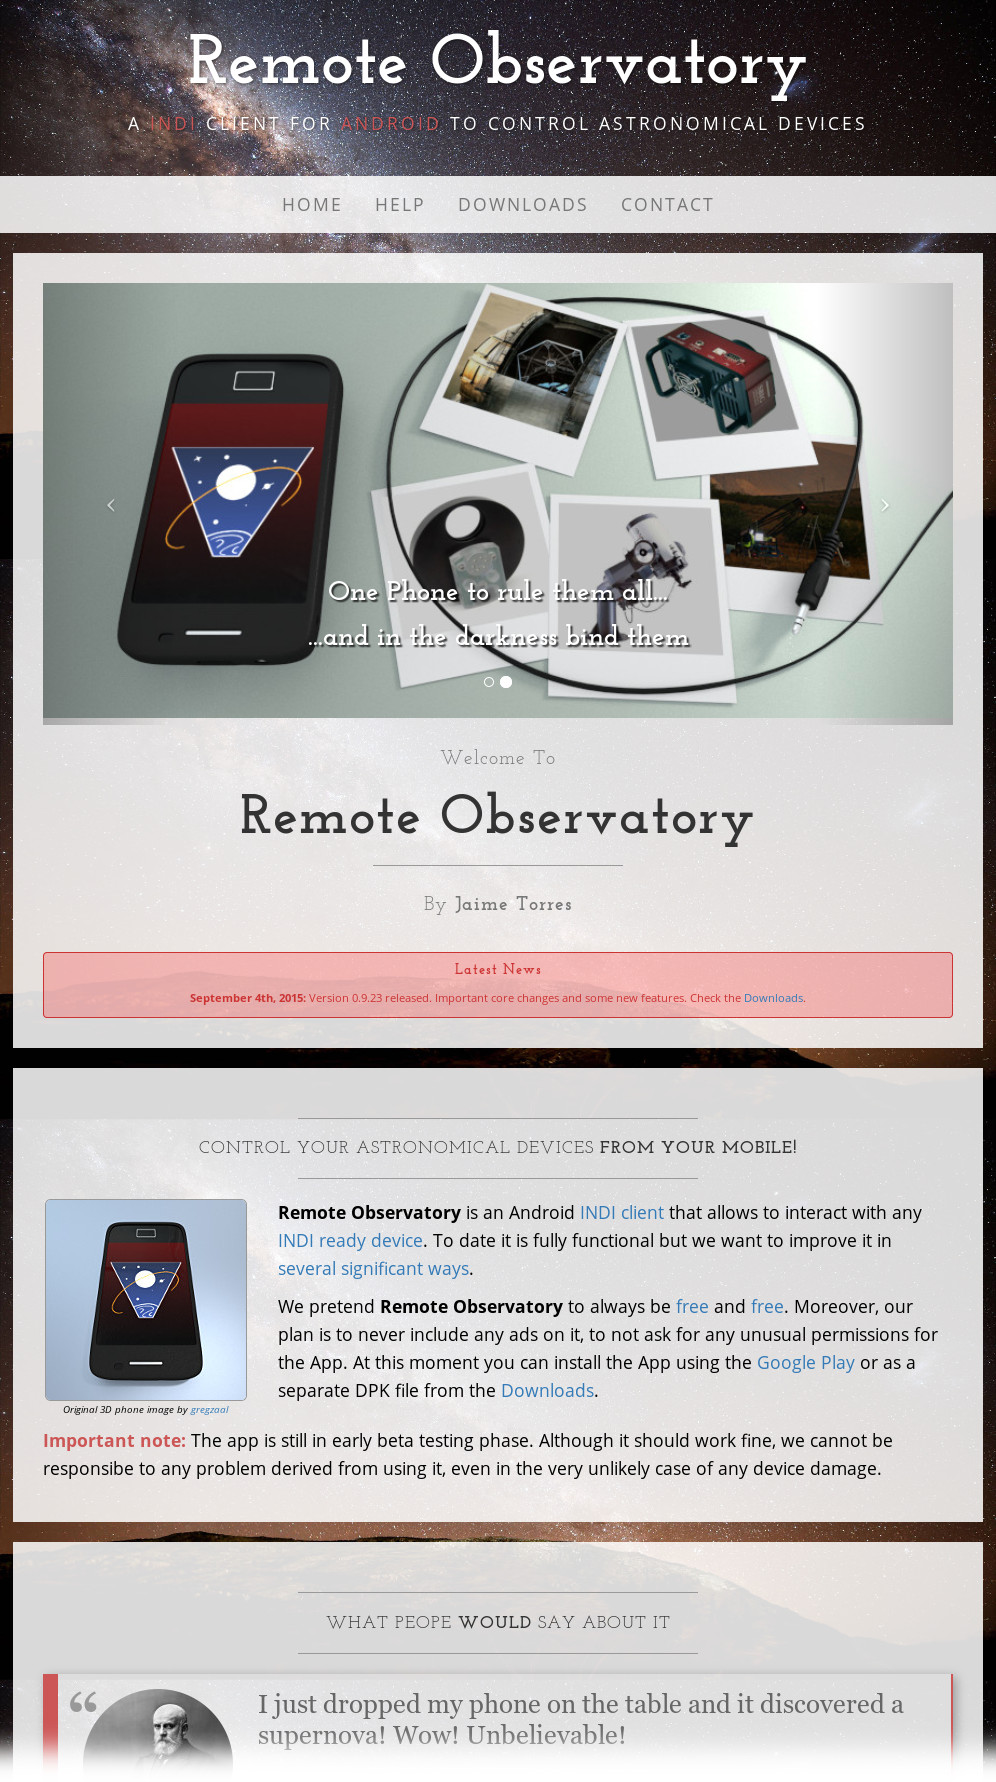
\includegraphics[width=12cm]{../images/webpage2.jpg}
 % webpage.jpg: 0x0 pixel, 300dpi, 0.00x0.00 cm, bb=
 \caption{Captura de la Página Web en Firefox (PC, Linux)}
 \label{fig:web}
\end{figure}

Se ha registrado el siguiente dominio: \url{http://remoteobservatory.info} así como contratado un hosting para poder crear una página web del proyecto (figura \ref{fig:web}). La idea principal de dicha página es dar a conocer la aplicación de un modo visual y atractivo. Aunque probablemente el público objetivo de la misma no necesite grandes alicientes visuales para decidir probarla, se e ha querido dar un diseño actual. Se han tenido en cuenta las siguientes consideraciones a la hora de crear dicho sitio web:

\begin{itemize}
  \item Crear un sitio claro, directo y con la información más relevante sobre la aplicación: descripción del proyecto, ayuda (incluyendo el manual de usuario) y una sección de descargas.
  
  \item Crear un sitio visualmente atractivo y \textit{responsive} para asegurarnos que se ve de manera adecuada tanto en ordenadores personales como en dispositivos móviles (figura \ref{fig:webMovil}).
  
  \item Ilustrar el sitio con algunas imágenes que intenten transmitir la idea fundamental del proyecto: poder controlar dispositivos astronómicos de manera sencilla desde un móvil.
  
  \item Ofrecer claramente información de contacto con el desarrollador de la aplicación para que sea fácil establecer canales de comunicación entre los usuarios y el mismo (indispensable para depurar errores y obtener ideas sobre posibles nuevas funcionalidades).
  
  \item Dotar a la página de ciertos toques de humor geek que probablemente saquen alguna sonrisa a los aficionados a la astronomía.
\end{itemize}


\begin{figure}
 \centering
 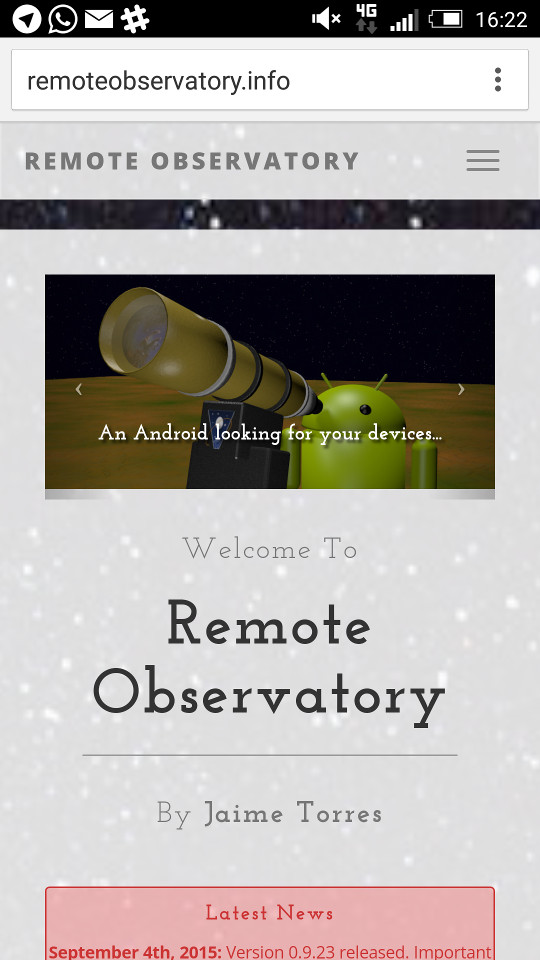
\includegraphics[width=6cm]{../images/webMovil.jpg}
 % webpage.jpg: 0x0 pixel, 300dpi, 0.00x0.00 cm, bb=
 \caption{Captura de la Página Web en Teléfono Móvil}
 \label{fig:webMovil}
\end{figure}

Para conseguir estos objetivos se ha optado por usar una plantilla basada en Bootstrap (http://getbootstrap.com/ ESTO SE PONE COMO BIBLIOGRAFÍA), uno de los frameworks HTML, CSS y JS más utilizados en la actualidad. Entre otras ventajas, permite desarrollar rápidamente un sitio web con un aspecto depurado en muy poco tiempo, especialmente si se utiliza una plantilla predefinida (que luego se modifica acorde al proyecto actual). En este caso, se utilizó una plantilla denominada Bussiness Casual (http://startbootstrap.com/template-overviews/business-casual/ OTRA BIBLIO).



\section{Publicación en Google Play}

\begin{figure}
 \centering
 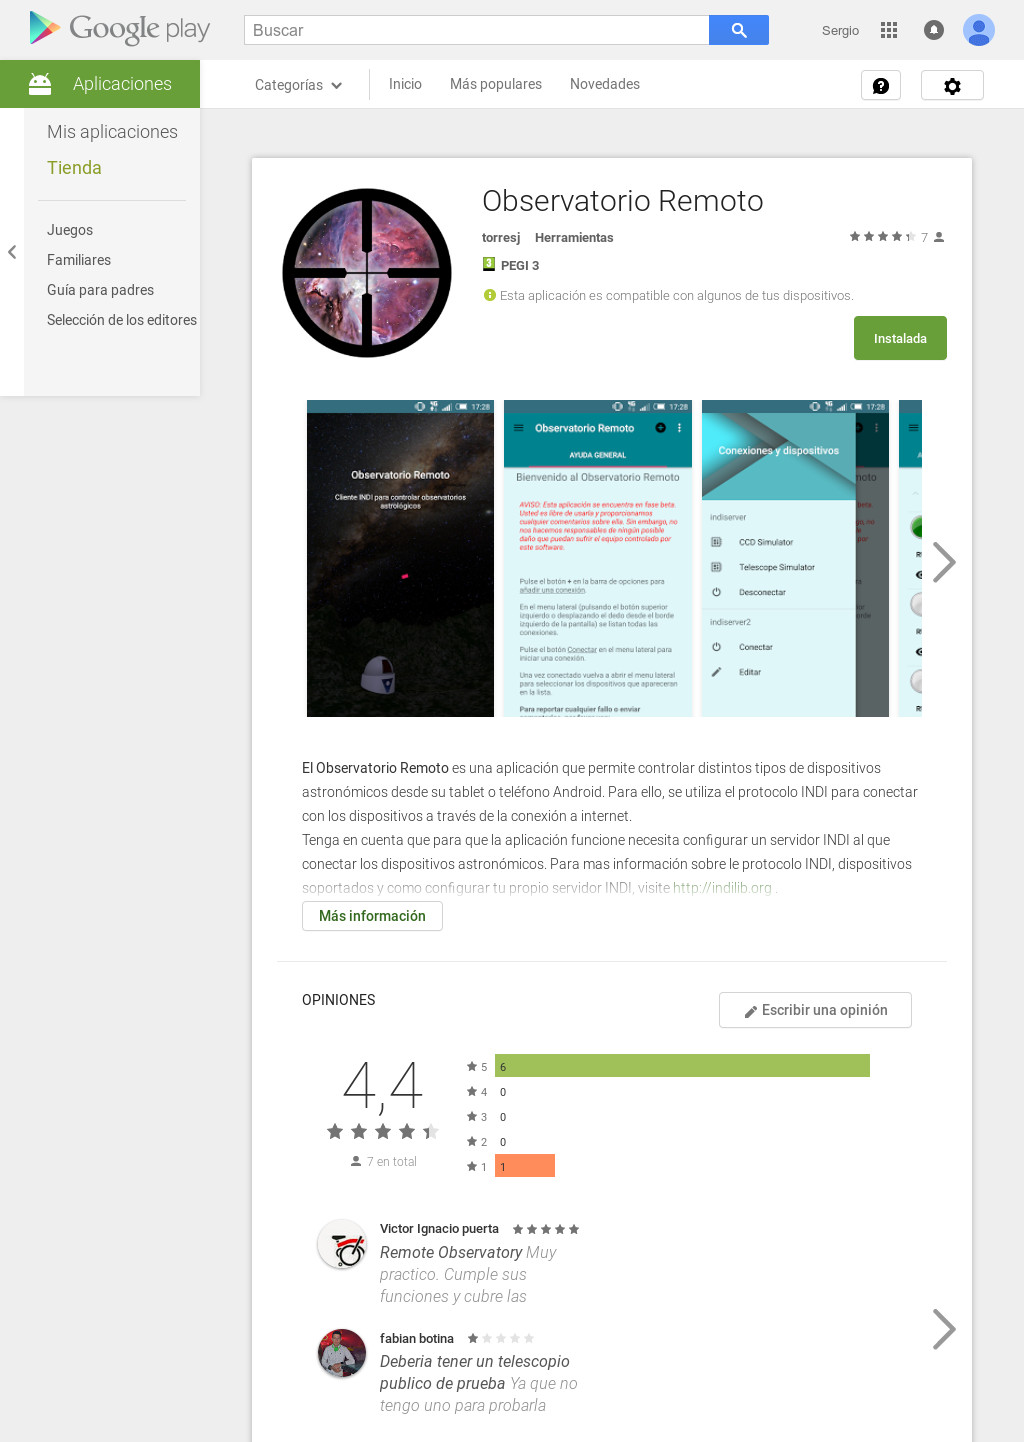
\includegraphics[width=12cm]{../images/googlePlay.jpg}
 % webpage.jpg: 0x0 pixel, 300dpi, 0.00x0.00 cm, bb=
 \caption{Captura de Remote Observatory en Google Play}
 \label{fig:googlePlay}
\end{figure}

La inmensa mayoría de los usuarios de Android instalan sus aplicaciones móviles utilizando la Google Play. Aunque otras vías de instalación son posibles (como la distribución del APK y su instalación manual), se ha creído conveniente añadir la aplicación a dicha tienda online (figura \ref{fig:googlePlay}). Evidentemente la aplicación ha sido publicada sin ningún coste y totalmente accesible. Se ha incluido en la categoría \texttt{Herramientas}. Se ha procurado poner una descripción clara de la aplicación para que los posibles usuarios sepan si les puede ser útil o no.

Es interesante reseñar que en el poco tiempo que lleva publicada la aplicación algunos usuarios desconocidos (con los que no se ha contactado por ningún otro medio de manera explicita) ya se han instalado la aplicación. También es digno de mencionar que un usuario ha calificado muy mal la aplicación porque considera que ``debería tener un telescopio público de prueba'', lo que pone de manifiesto que siempre podemos encontrar gente dispuesta a pedir absolutamente de todo.

\section{Mantenimiento del Repositorio en GitHub}

Dado el carácter libre de la aplicación, todo el código de la misma está ubicada en un repositorio en GitHub (https://github.com/ BIBLIOGRAFÍA). La dirección de dicho repositorio es la siguiente: \href{https://github.com/torresj/indi-android-ui}{https://github.com/torresj/indi-android-ui}. Como es habitual en este tipo de repositorios, se encuentran mecanismos que permiten inspeccionar el código, descargarlo, comparar cambios, contactar con el desarrollador, gestionar tickets, etc.

Además, a misma plataforma se puede ver como un mecanismo de difusión para que otros desarrolladores interesados en la temática astronómica puedan interesarse por la aplicación y el proyecto en general (lo que podría atraer otros desarrolladores).

\section{Difusión en la Página Oficial de la Biblioteca INDI}

Dado que la gran mayoría de los potenciales usuarios de la aplicación conocerán el protocolo INDI y es probable que visiten su sitio web oficial (http://indilib.org), nos hemos puesto en contacto con sus encargados para que añadieran esta aplicación como uno de los posibles clientes INDI existentes. Al poco actualizaron la página web del proyecto incluyéndolo (figura \ref{fig:indiLibWeb}).


\begin{figure}
 \centering
 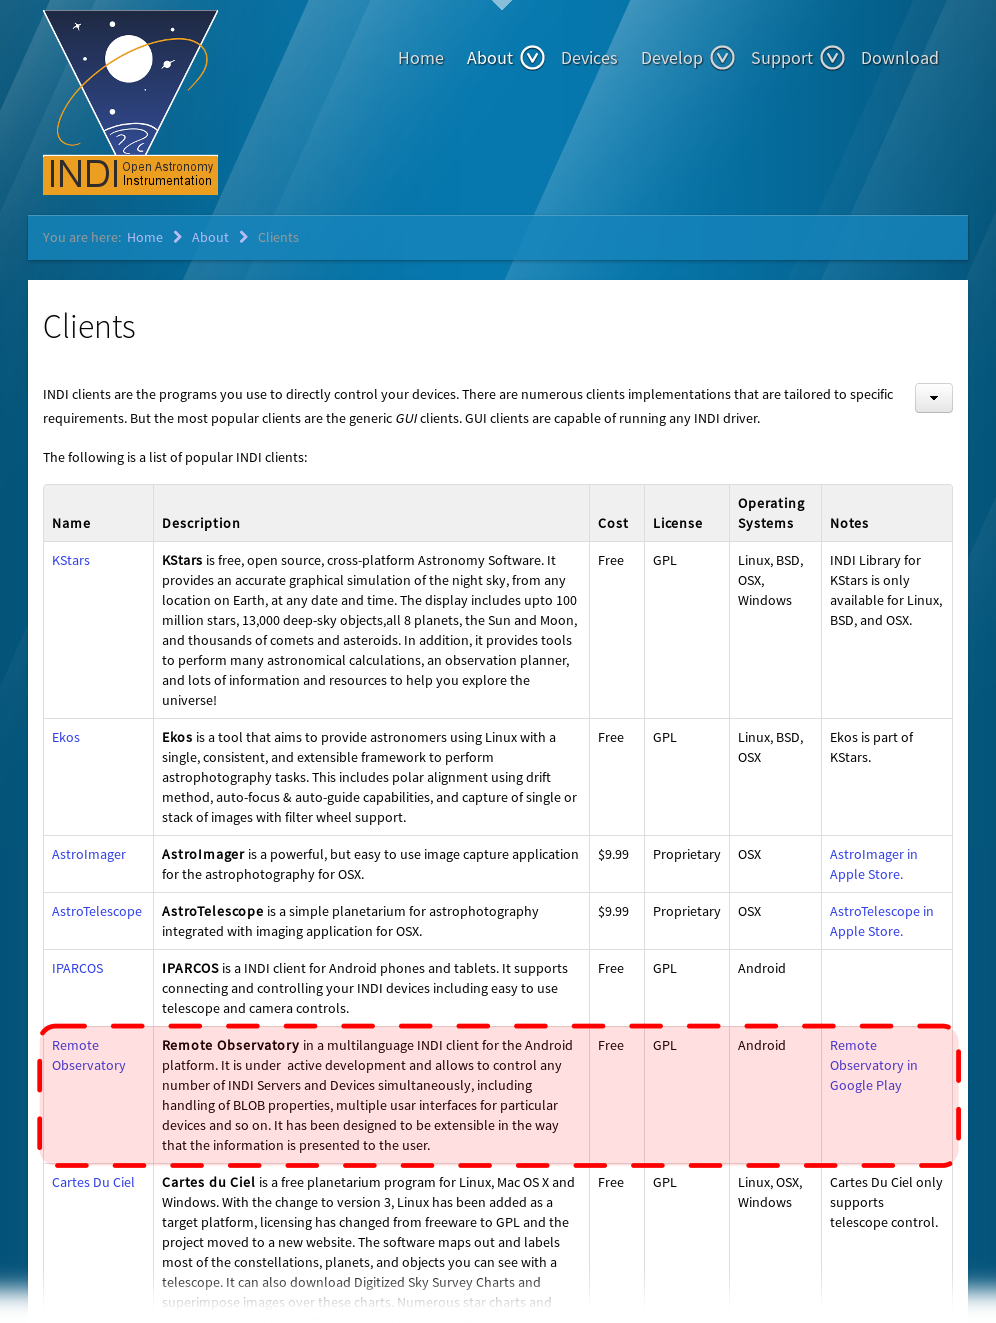
\includegraphics[width=12cm]{../images/indilibWeb3.png}
 % webpage.jpg: 0x0 pixel, 300dpi, 0.00x0.00 cm, bb=
 \caption{Captura de la página web oficial de la biblioteca INDI, donde se menciona al Observatorio Remoto \protect\href{http://indilib.org/about/clients.html}{http://indilib.org/about/clients.html}}
 \label{fig:indiLibWeb}
\end{figure}



\section{Difusión en el Foro Oficial de la Biblioteca INDI}

La página oficial de la biblioteca INDI tiene un foro donde se discuten temas relacionados: desde problemas con el uso de la biblioteca o alguna de sus herramientas relacionadas, se discuten temas de actualidad astronómica o detalles de implementación de la biblioteca, de los drivers, etc.

Se ha creado un hilo específico en el foro anunciando la aplicación (figura \ref{fig:indiForum}) lo que ha provocado que algunos usuarios se interesen y hayan empezado a mandar comentarios e incluso algún informe de errores.

\begin{figure}
 \centering
 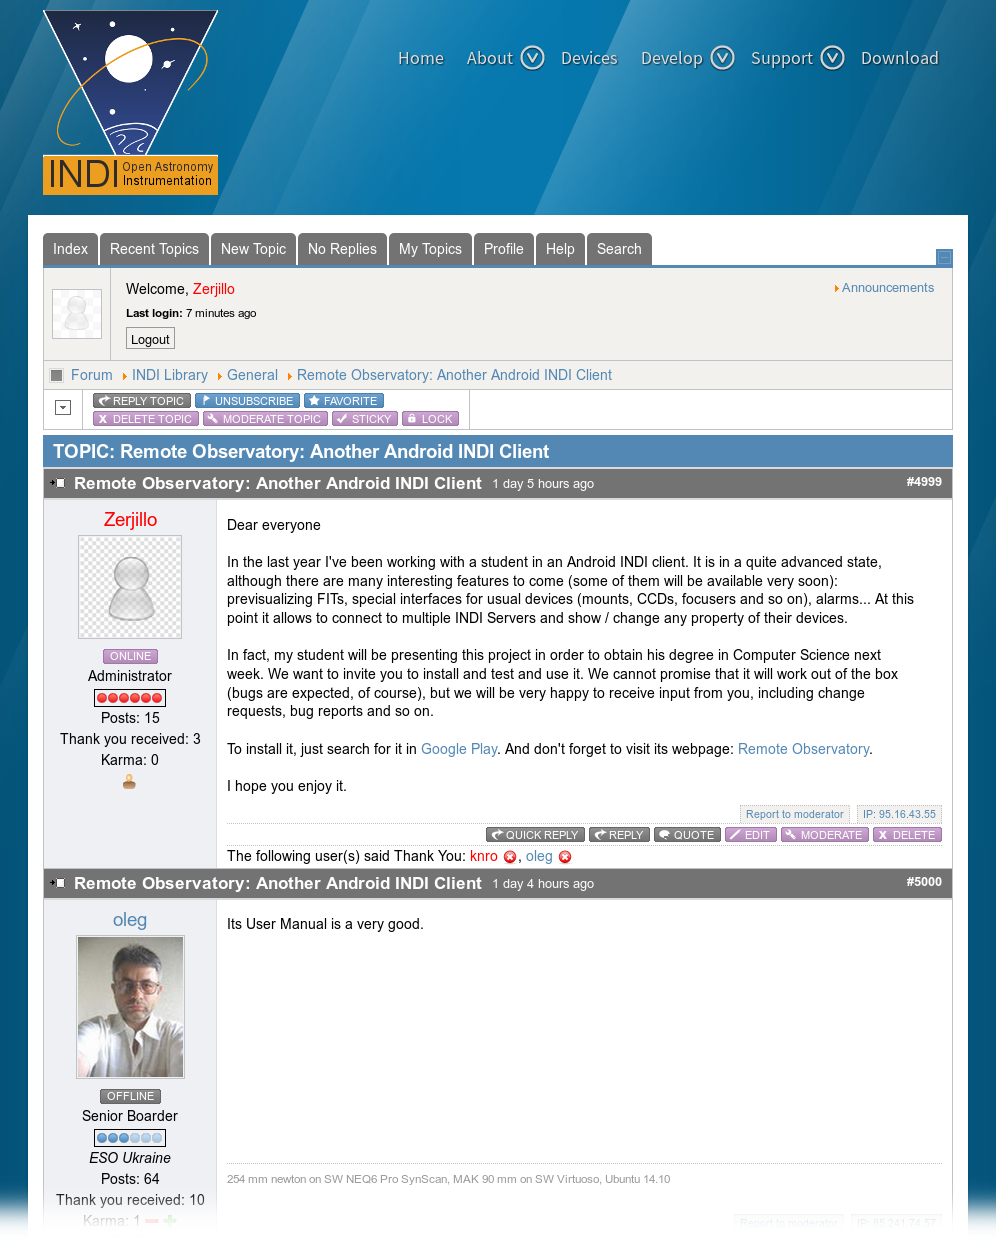
\includegraphics[width=12cm]{../images/indiForum2.png}
 % webpage.jpg: 0x0 pixel, 300dpi, 0.00x0.00 cm, bb=
 \caption{Captura del hilo del foro de la biblioteca INDI donde se presenta la aplicación \protect\href{http://indilib.org/forum/general/823-remote-observatory-another-android-indi-client.html}{http://indilib.org/forum/general/823-remote-observatory-another-android-indi-client.html}}
 \label{fig:indiForum}
\end{figure}



\section{Algunas Ideas Futuras Para La Difusión}

Además de las actividades comentadas, se tienen planeadas algunas más para realizar en un futuro no muy lejano y aumentar la visibilidad del proyecto. Entre otras nos gustaría mencionar:

\begin{itemize}
  \item Creación de un vídeo demostrativo de la aplicación y su uso con instrumental astronómico real. Además, este vídeo puede usarse para incrustarse tanto en la página web de la aplicación con en la página de Google Play.
  
  \item Poner a disposición del público un servidor INDI que implemente los simuladores de telescopio básicos para que los usuarios puedan hacer algunas pruebas fácilmente aunque no dispongan de hardware astronómico.
\end{itemize}